\subsection{Experiment Interfaces}

\subsubsection{Mechanical Interfaces}
\label{sec:4.2.1}

\colorbox{red}{AN UPDATED CAD WILL BE MADE BEFORE JAN 16TH}\\
\colorbox{orange}{\parbox{\textwidth}}{THIS SECTION WILL BE FINALISED WHEN AN UPDATED CAD MODELAND INTERFACE DESIGN WILL BE AVAILABLE}\\
The experiment mounting platform will be attached to the upper rails of the gondola.

% Discuss mounting safety


\begin{figure}[H]
    \centering
	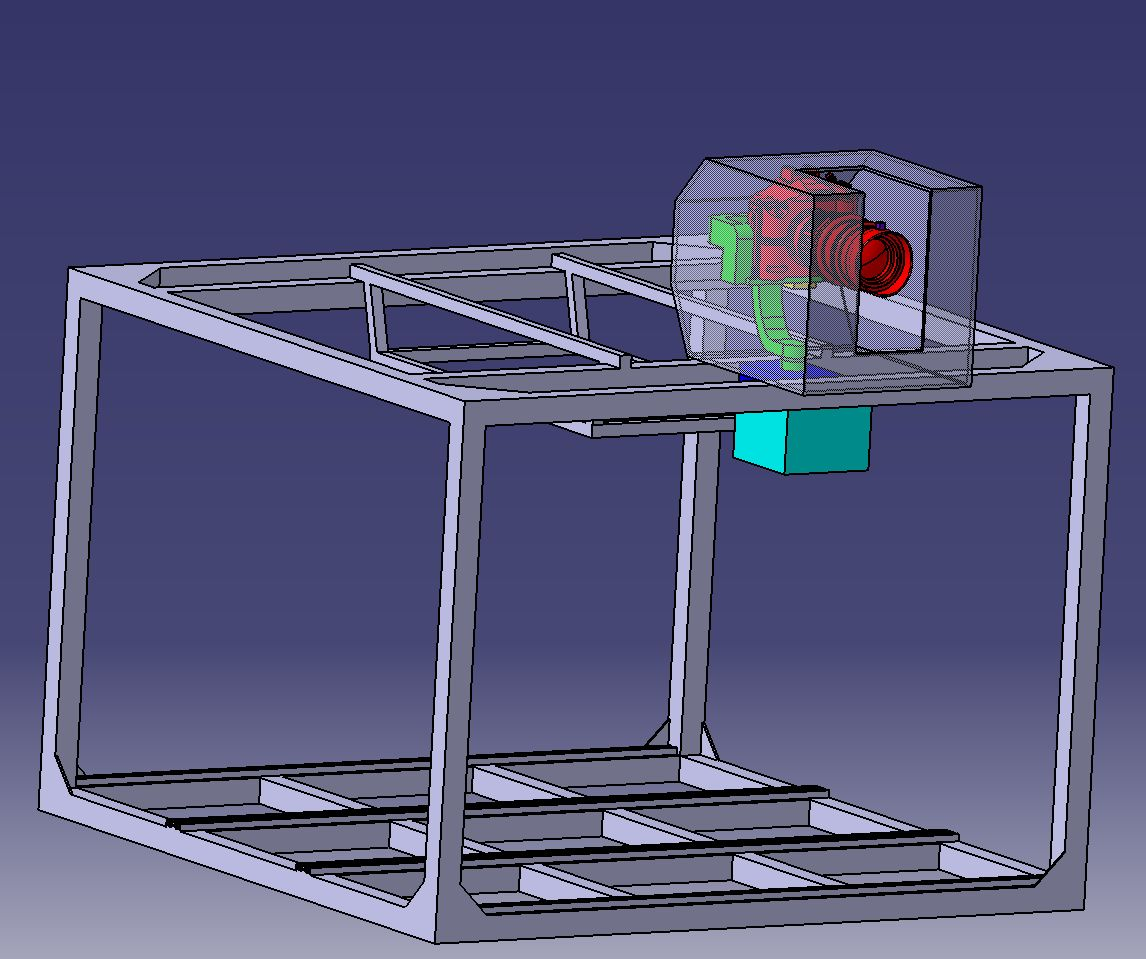
\includegraphics[width=0.5\linewidth]{4-experiment-design/img/interfaces/Screenshot_Experiment.jpg}
	\caption{Instrument position on gondola}
\end{figure}

\begin{figure}[H]
    \centering
	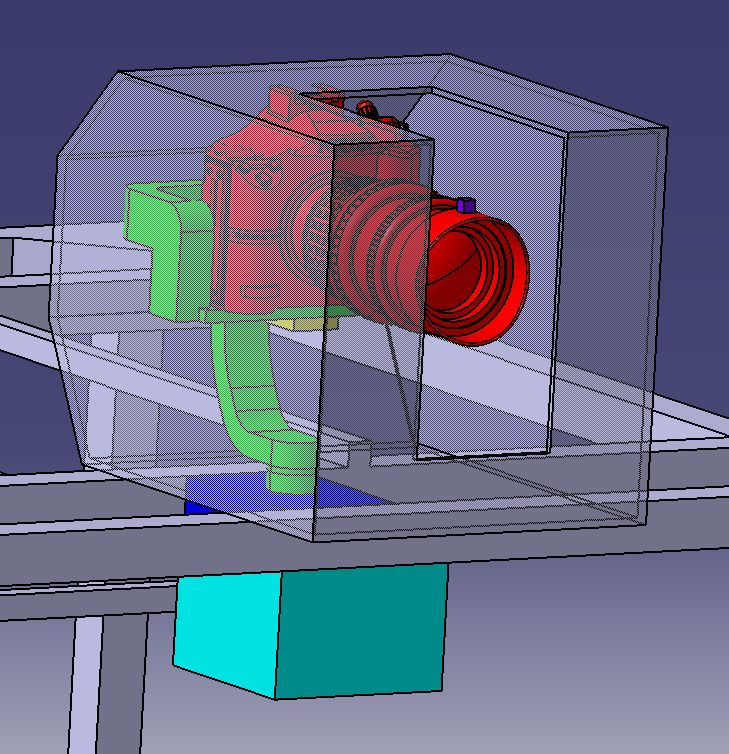
\includegraphics[width=0.5\linewidth]{4-experiment-design/img/interfaces/Screenshot_Close_Up.jpg}
	\caption{Close up of the instrument mounting}
\end{figure}


% \bigskip
% \input{4-experiment-design/tables/attaching_comp.tex}


\subsubsection{Thermal Interfaces}
    \colorbox{orange}{\parbox{\textwidth}}{THIS SECTION REQUIRES THERMAL ANALISYS AND DESIGN}\\
The IRISC experiment will be shielded from heat transfer.
\label{sec:4.2.2}


\subsubsection{Electrical Interfaces}
\label{sec:4.2.3}
\textbf{E-link:}\\
The uplink will be used to send occasional commands to control the experiment. One command will be [\hl{TBD}] in size. The TCP/IP protocol will be used for uplink, so the total size of one transmission will be the data plus the TCP header (maximum 480 bits), the IP header (maximum 480 bits) and the Ethernet frame (144 bits). 

$$ bits\, per\, uplink\, packet \leq [TBD] + 480 + 480 + 144 $$

The downlink will be used to send science and housekeeping data to the ground station. The data in the downlink packet is estimated to be [\hl{TBD}]. For downlink, UPD protocol will be used, as the reliability of the data is not as crucial as during the uplink and to compensate for the size of the data packet. The total size of one packet will be the data plus the UDP header (32 bits), the IP header (maximum 480 bits) and the Ethernet frame (144 bits).

$$ bits\, per\, downlink\, packet \leq [TBD] + 32 + 480 + 144 $$

\textbf{Power:}\\
Power will be delivered to the electric box from the provided 28.8 V/1 mA (13 Ah) battery pack. Only one pack is required. The expected minimum current is [\hl{TBD}], the average is [\hl{TBD}] and the maximum is [\hl{TBD}].

\textbf{Connectors:}\\
The power cable are attached as it can be seen on Figure \ref{fig:power_cables}, and the E-link cables are attached as on Figure \ref{fig:elink_cables}.

\begin{figure}[H]
    \centering
	\includegraphics[width=0.2\linewidth]{4-experiment-design/img/interfaces/power_cables.jpg}
	\caption{Position of power cable socket}
\end{figure}

\begin{figure}[H]
    \centering
	\includegraphics[width=0.2\linewidth]{4-experiment-design/img/interfaces/elink_cables.jpg}
	\caption{Position of E-link cable socket}
\end{figure}


\textbf{Protection:}\\
The PSU shall have and overcurrent protection in form of a fuse. Moreover, a manual killswitch shall be installed and be available to reach without taking apart the electronics casing.

\textbf{Grounding:}\\
Each electronic subsystem will be connected to a single point ground.


% \subsubsection{Radio Frequencies (Optional)}



\raggedbottom